
\documentclass{uonmathreport}

% this allows one to include .jpg etc figures using pdflatex
% change the optional argument if you use dvips or others
\usepackage[pdftex]{graphicx}
\usepackage[utf8]{inputenc}
\usepackage[english]{babel}
\usepackage{amsthm}
\usepackage{float}
\usepackage{hyperref}
\usepackage{algorithm,algcompatible}
\usepackage{listings}
\usepackage{color}


\definecolor{codegreen}{rgb}{0,0.6,0}
\definecolor{codegray}{rgb}{0.5,0.5,0.5}
\definecolor{codepurple}{rgb}{0.58,0,0.82}
\definecolor{backcolour}{rgb}{0.95,0.95,0.92}
 
\lstdefinestyle{mystyle}{
    backgroundcolor=\color{backcolour},   
    commentstyle=\color{codegreen},
    keywordstyle=\color{magenta},
    numberstyle=\tiny\color{codegray},
    stringstyle=\color{codepurple},
    basicstyle=\footnotesize,
    breakatwhitespace=false,         
    breaklines=true,                 
    captionpos=b,                    
    keepspaces=true,                 
    numbers=left,                    
    numbersep=5pt,                  
    showspaces=false,                
    showstringspaces=false,
    showtabs=false,                  
    tabsize=2
}
 
\lstset{style=mystyle}




\DeclareMathOperator*{\argmax}{\arg\!\max}% https://tex.stackexchange.com/q/83169/5764
\algnewcommand\INPUT{\item[\textbf{Input:}]}%
\algnewcommand\OUTPUT{\item[\textbf{Output:}]}%
% other packages that maybe of use include:
% hyperref, amsthm, xy, todonotes, showkeys, ...
\newtheorem{definition}{Definition}[section]
\newtheorem{theorem}{Theorem}[section]
\newtheorem{lemma}{Lemma}[theorem]

% change to \PJS or \DIS or \HGDIS (for BSc and MPhil)
% or \MSc (for all Msc dissertations)
\PJA

% adjust the following
\title{A quantitative approach to Consistency Theorem in Clustering}
\author{Zehui Li}
\academicyear{2018/19}
\supervisor{Dr. Yves van Gennip}

% the following are irrelevant for Msc:
\assessmenttype{Review} % or Investigation
\projectcode{XX P99}


% gives double-spacing
\linespread{1.6}
% the margins are set automatically. Do not make them smaller.

% put your own definitions and shorthands here
\newcommand{\ZZ}{\mathbb{Z}}

\begin{document}

\maketitle

\begin{abstract}
Various Clustering Algorithms are usually studied independently, however, in 2003, Kleinberg\cite{Kleinberg} proposed three properties called \textbf{Scale-invariance}, \textbf{Richness} and \textbf{Consistency}, which are universally applied to all the clustering algorithms. In this paper, we review Kleinberg's work, then taking a numerical analysis approach to study the \textbf{Consistency} property. It mainly has three contributions. Firstly, this paper provides a complete review of Kleinberg's paper, and gives proofs for three theorems about Single-linkage algorithm. Secondly, we point out problems with consistency property. Finally, through the simulation, we identify the skewed distribution of Adjusted Rand Index on the $\Gamma$-transformed dataset. This skewed distribution indicates that for the algorithms that don't satisfy the consistency property, they still exhibit the property similar to consistency, we defined this weak version of consistency as \textbf{Partial Consistency}.

\end{abstract}

% Table of contents
\setcounter{tocdepth}{2}  % this will list subsections, but not subsubsections
\tableofcontents 
\newpage

\section{Introduction} \label{sec:intro}
\subsection{Background}
Clustering analysis can be defined as a process of segmenting the data points into several subsets, or clusters, with the goal of making the data points within a cluster to be similar to each other, while the data points in distinct clusters to be different. Clustering has been widely used in many fields, such as pattern recognition, bio-informatics and image processing, however, most of the study toward the uniform notion of clustering only stop at the very general level. The algorithms doing the clustering analysis are called \textbf{clustering algorithm}, depending on the definition of the clusters and the way to find the clusters, these clustering algorithms differ from each other significantly. In 2003, Kleinberg \cite{Kleinberg} published a highly influential paper, in which he set up a general framework to study clustering algorithms as a whole, and proposed three properties that any clustering algorithms could have.

Clustering algorithms fall into three categories \cite{esl}: combinatorial algorithms, mixture modelling, and model seeking, the algorithms in each category follows different underlying principal. The advantage of Kleinberg's framework is that it can be applied to all these clustering algorithms regardless of these principal. The core of the framework - three properties proposed by Kleinberg - are called \textbf{scale invariance}, \textbf{richness} and \textbf{consistency} respectively. \textit{Scale invariance} states that if the distance (dissimilarity) between the data points is multiplied by a positive number, the clustering algorithm should partition the data into the same clusters as before. \textit{Richness} requires that for any given partition of the data points, it will be possible to come up with a pair wise distance between the data points, so that the clustering algorithm can produce the given partition. Finally, a clustering algorithm satisfy the \textit{consistency property} if we apply $\Gamma$-transformation\footnote{The definition of $\Gamma$ transformation is defined in section \ref{subsec:priliminaries}. Basically, $\Gamma$-transformation is a specific way to perturb dataset by decreasing the distance between the data points within a cluster, increase the distance between the clusters} on original dataset, the algorithm can produce the same partition on this new dataset. The most important conclusion from Kleinberg's paper is that there is no clustering algorithm which could satisfy three properties at the same time.

\subsection{Methods and structure of the paper}

Following the impossibility theorem proposed by Kleinberg, numerous relaxation methods on the axiomatic system are proposed in recent years. In particular, relaxation of consistency property is often suggested. The consistency theorem proposed by Kleinberg, while reasonable and simple, it give a relative strict restriction on clustering algorithms - it require the clustering algorithm to give the same partition results even when the data set is perturbed profoundly (we will explain why this theorem is not sensible in more details next section). With this in mind, we simulate the $\Gamma$-transformation process: Python is used to implement the simulation, and Adjusted Rand Index is used as a criteria to compare the difference between two partition results. Through the simulation, we found that some clustering algorithms will have the tendency to produce the same partition results on $\Gamma$-transformed dataset. We define this property as ``Partial Consistency". 

In this paper, we start from reviewing the work of Kleinberg, adding the missing proofs to three theorems about Single-linkage clustering algorithm, then point out the potential problem with consistency. After these work, the rest of the paper will focus on the study of consistency theorem - we come up with a quantitative framework to investigate the property of $\Gamma$-transformation, and identify the highly separable distribution of partition results given legitimate perturbation. Finally, we tried several machine learning methods to predict whether the clustering algorithm can produce the same partition on $\Gamma$-transformed datasets.

\section{Review of Kleiberg's work} \label{sec:background}
This section begins by introducing the mathematical notations used for clustering, and give the formal definition of scale invariance, richness and consistency theorem. After having these knowledge in mind, we will move on to prove three statements about a very simple clustering algorithm - single linkage. In the third subsection, we will discuss why consistency theorem  is a more strict restriction compared to the others, Which gives us motivation to explore the ways to change consistency theorem.
\subsection{Priliminaries} \label{subsec:priliminaries}
Every clustering algorithm can be denoted by a ``clustering function" $f$, the input of this function is a set $S$ consisting of $n$ data points and the pairwise distances among them. Each points in set $S$ is represented by a integer, so $S = \{1,2,3,...,n\}$ with $n>=2 $. There are multiple ways to represent the pairwise distances, for example, for $S = \{1,2,3,...,N\}$, a $N \times N$ distance matrix $M$ can be used to represent the distances, in which each entry $M_{i,j}$ refer to the distance between points $i$ and $j$. However, in our case, instead of using the distance matrix, we will use \textit{distance function} to denote the pairwise distances, which is more convenient when dealing with the theorems we defined below. \textit{Distance function} is define as a function $d$: $S \times S \rightarrow \mathbb{R}_{\ge 0}$ with symmetric property, thus, $d(i,j)$ equals $d(j,i)$, and both represent the distance between the points $i,j \in S$. In particular, $d(i,i) = 0$ for any $i\in S$. Distance function are not required to be \textit{metrics}, in other words, $d$ doesn't need to satisfy triangle inequality, but adding such restriction will not affect results we have below.

Naturally, \textit{clustering function} $f$ take a data Set $S$ and a distance function $d$ as the inputs, and output the a partition $\Gamma$ of $S$, where $\Gamma = \{C_1,C_2,...,C_k\}$, each of the non-overlap subsets $C_k$ contains some of the data points in $S$. For example, let $S = \{1,2,3,4,5\}$, then we could have $f(S,d)= \Gamma = \{ \{1,2\},\{3,4,5\} \}$. For simplicity, we can also write $f(S,d)$ as $f(d)$ without explicate referring to data set S. These three properties - scale invariance, richness and consistency - are all defined around this clustering function $f$.

\begin{definition}
Scale-Invariance. $f$ satisfy Scale-Invariance $\iff$  For any given distance function $d$ and any $\alpha>0$, $f(d) = f(\alpha\cdot d)$
\end{definition}

Scale Invariance simply requires that the clustering algorithm don't rely on the fixed quantity to cluster the dataset.

\begin{definition}
Richness.  $f$ satisfy Richness $\iff$ For any given partition $\Gamma$ of $S$, $\exists d$ such that $f(d) =\Gamma$
\end{definition}

This property is called richness, because the by feeding in the clustering algorithm different distance functions $d$, we can reach any possible partition of the given data set $S$. The third property is called consistency, and it contains more details than the first two. The basic idea of consistency is that, if we perturb the data in a desirable way, our algorithm should produce the same partition $\Gamma$. We first give a formal definition to the ``desirable perturbation", calling it $\Gamma$ \textit{-transformation}.
\begin{definition}
Given a partition $\Gamma=\{C_1,C_2,...,C_m\}$ on data set $S$, 
$d'$ is a $\Gamma$ \textit{-transformation} of $d$ $\iff$ For any points $i,j\in C_k$, $d'(i,j)<=d(i,j)$; and if $i \in C_k, j\notin C_k$, $d'(i,j)>=d(i,j)$.
\end{definition}

It may seems a little messy at the first glance, but we can interpret $\Gamma$ \textit{-transformation} as a specific way to perturb the dataset. Suppose we have a data set at the beginning, then we apply a clustering algorithm on this data set, and obtain several clusters. We will squash the points within the same cluster together, and move the points in one cluster away from the other clusters. The resulting distance, will be $d'$ in our definition above. And consistency property simply require that, if we apply the clustering algorithm on the perturbed version of data set, we will still have the same points assigned to the same clusters.

\begin{definition}
Consistency. f satisfy consistency $\iff$ Given that $d'$ is $\Gamma \textit{-transformation}$ of distance function $d$, $f(d) = f(d')$
\end{definition}

Kleinberg's framework starts from abstraction: it abstracts clustering algorithm into a clustering function $f$, then defines several properties to analyse the function. Once we have this framework, there are two direction to continue the study: the first is to come down to specific algorithms and study whether or not this clustering algorithm satisfy these properties; the other way is to modify the existing properties or add new properties into this framework. Both approaches are mentioned in this paper: We study \textbf{single linkage} clustering algorithm in the next section, then the rest of the paper will seek ways to modify the \textbf{consistency} theorem.
\subsection{Missing Proofs for single linkage} \label{subsec:Single-linkage}

Single-linkage is a bottom-up hierarchical clustering algorithm, it begin with each clusters representing a single group, then at each step, it will merge the two ``nearest" (with least dissimilar) clusters into a single cluster, where dissimilar is defined in following manner \cite{esl}. The algorithm will terminate until some termination condition is satisfied.
\begin{definition}
Let G,H represent two clusters, d is the distance function of the data set, then dissimilar $d_{SL}$ is defined as:
$d_{SL}(G,H) = \min_{i\in G,i'\in H}d_{ii'} $
\end{definition}

An alternative way to describe Single-linkage is to treat clustering as a Graphs Construction process \cite{christopher2008introduction}. Tuple $(S,d)$ naturally form a complete Graph $G(S,d)$, whose node set is  the data set $S$, and weigh of edges between nodes $i,j \in S$ is the distance function $d_{ij}$. Single linkage will first order the edges in the non-decreasing order, then for each iteration, it will take one edge from the ordered list,then terminate when the termination condition is satisfies. At this point, all the picked edges form a new partially connected graph $G_{c}$, where the node set is the still the data set, but edge set is a set formed by all picked edges. We will use this graph perspective in the following proofs.

By controlling the "termination conditions", we can construct three single linkage algorithms, such that each of the them can satisfy two properties out of Scale-invariance, Richness and Consistency. Three stop conditions are listed below\cite{Kleinberg}.
\begin{itemize}
\item \textit{k-cluster termination condition}. Stop adding edges when the partially connected graph $G_{c}$ consists of k connected components.
  
\item \textit{distance-r termination condition.} Only add edges of weight at most r.
  
\item \textit{scale-$\alpha$ termination condition.} Let $\rho^*$ denote the maximum pairwise distance; i.e $\rho^* = \max_{i,j}d(i,j)$. Only add edges of weight at most $\alpha\rho^{*}$.
\end{itemize}

Each of the termination condition is a trade-off between three properties: for example, single linkage with \textit{distance-r} termination condition has a built-in scale, so it will not satisfy the scale-invariance property. But this algorithm indeed satisfy Richness and Consistency. Similarly, we have the following theorem:
\begin{theorem}
\label{first theorem}
For any $\alpha>=1$, and any $n>=3$, single-linkage with the scale-$\alpha$ termination condition satisfies Scale-Invariance and Richness.
\end{theorem}
\begin{theorem}
\label{second theorem}
For any $k>=1$, and any $n>=k$, single-linkage with the k-cluster termination condition satisfies Scale-Invariance and Consistency.
\end{theorem}
\begin{theorem}
\label{third theorem}
For any $r>0$, and any $n>=2$, single-linkage with the distance-r termination condition satisfies Richness and Consistency.
\end{theorem}

Here we present the proof of \textit{Theorem 2.1} and enclosed the proof of \textit{Theorem 2.2} and \textit{2.3} in the appendix \ref{app:proof}

\begin{proof}
\label{pf:myproof1}
\textit{theorem \ref{first theorem}}

\noindent Given data set $S$ and distance function $d$, let $\rho^* = \max_{i,j}d(i,j)$, and $f$ be the single-linkage with scale-$\alpha$ termination condition. 

Let's first prove that $f$ satisfy Scale-invariance property. Assume another distance function $d'$, and $d'$ satisfy that for $\forall$ $i,j \in S, d'(i,j)=\beta d(i,j)$, where $\beta >0$. Let $\Gamma = f(S,d)$, $\Gamma' = f(S,d')$ respectively. If we can show that $\Gamma = \Gamma'$, we will prove $f$ satisfy Scale-invariance. Following the Graph interpretation of single-linkage, the resulting partition can be represented by a partially connected Graph $G_c(S,E)$, where the node set is data set $S$, and edge set $E$ consists of picked edges. Let $G_c(S,E) = \Gamma = f(S,d)$, and $G_c'(S,E') = \Gamma' = f(S,d')$. Now, if we can prove that $G_c(S,E) = G_c'(S,E')$, we are done. To prove $G_c' = G_c$, we only need to prove that edge set $E=E'$, because $G$ and $G'$ have the same node set.

Let's look inside $E$ and $E'$: Due to ``scale-$\alpha$" termination condition, edge Set $E$ will contain all the edges which has weights smaller than $\alpha\rho^*$. Formally, $d(e_i) <=\alpha\rho^*$, for $e_i\in E$; $d(e_j) > \alpha\rho^*$, for $e_j\notin E$. Similarly, $E'$ will only contain the edges which are smaller or equal to the ``threshold value", let's denote this value by $\rho_{2}^{*}$. So for $e_i \in E'$, $d'(e_i)<=\rho_{2}^{*}$, and for $e_j \notin E'$, $d'(e_j)>\rho_{2}^{*}$. But $d'(.) = \beta d(.)$ and $ \rho_{2}^{*} =  \max_{i,j}d'(i,j)= \max_{i,j}\beta d(i,j)=\beta \max_{i,j} d(i,j) =\beta\rho^*$. If we substitute the values of  $d'(e)$ and $\rho_{2}^{*}$ with $\beta d(e)$ and $\beta \rho^{*}$ in the inequality for $E'$, we will have $\beta d(e_i) <=\beta \alpha\rho^*$, for $e_i \in E'$, which is equivalent to the constraints for elements in $E$, thus $E'$ has the same elements as $E$, which indicate that $\Gamma = \Gamma'$, and we are done with the proof of Scale-invariance.

The proof for richness is much easier: Given a partition $\Gamma$, if we can construct a distance function $d$ such that $f(d) = \Gamma$, we are done. Let's assume we are given a partition $\Gamma = G_c(S,E)$, where $E = \{e_1,e_2,\ldots e_m\}$. To make $f$ produce such a edge set, we can define d as following: \[   
d(e_i) = 
     \begin{cases}
       \alpha^2, &\quad i\in\{1,2,3,\ldots m\} \\
       1, &\quad i\notin\{1,2,3,\ldots m\} \\
     \end{cases}
\]
In this manner, $\rho^{*} = \max_{i,j}d(i,j) = 1$, because \textit{theorem 2.1} assumes $\alpha<1$. Let $f(d) = G(S,E_{new})$, $f$ will put all the elements which are smaller and equal to $\alpha \rho^{*} = \alpha$ into $E$. Because $d(e_i)= \alpha^2 < \alpha$, for $i = 1,2\ldots m$, we have $E_{new} = \{e_1,e_2\ldots e_m\}=E$ 
\end{proof}


In this proof, we show how to prove Scale-invariance and Richness. The way to prove Consistency is somewhat similar to Scale-invariance, it starts from treating the partition $\Gamma$ as a partially connected Graph $G_c(S,E)$, then use the property of $f$ and the relation between $d$ and $d'$ to build the equivalence of two edge set $E$ and $E'$. The details are put in Appendix \ref{app:proof}.


\subsection{Why modify the consistency property?} \label{subsec: motivation for modifying consistency}
Kleiberg's \textbf{impossibility theorem} states that it is impossible for any clustering algorithm to have three properties at the same time, in other words, it indicates that we shoud not have unrealistic expectation to have a ``perfect“ clustering algorithm, but are these three properties desirable? Following the discussion in the blog of Willians\cite{williams_2015}, we will argue that, consistency property doesn't really reflect our expectation to clustering algorithm.

The idea of consistency theorem is that after we apply $\Gamma$-transformation to the data set, the clustering algorithm is not influenced by this perturbation, and can still produce the same partition results. As \textit{figure \ref{fig:bsd1}} illustrate, this property seem very intuitive at first glance: if we increase the distance between each cluster or squeezing the points within a cluster together, it should be more obvious to the algorithm that which points should be classified into the same group.
\begin{figure}[H]
 \begin{center}
   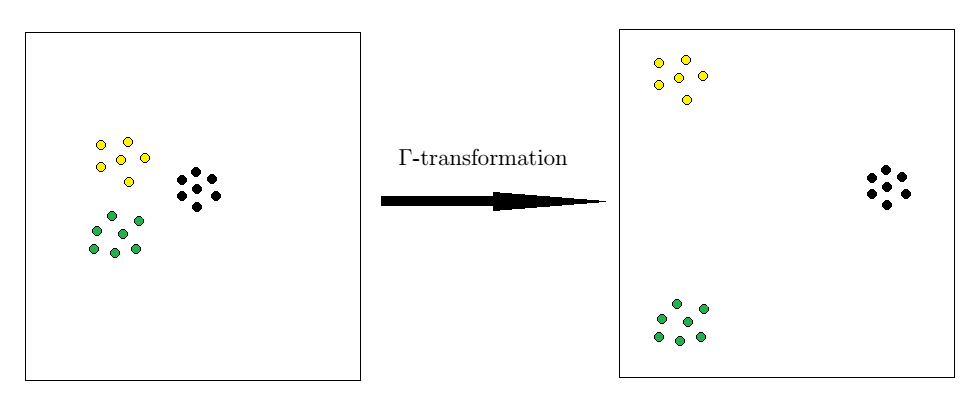
\includegraphics[width=0.75\textwidth]{Paper_figure_1.png}
 \end{center}
 \caption{\textit{This is example of $\Gamma$-transformation for two dimensional data: After the transformation the data points in different clusters are moved away from each other, and the boundary between ``clusters" should be more clear than before.}}
 \label{fig:bsd1}
\end{figure}

\begin{figure}[H]
 \begin{center}
   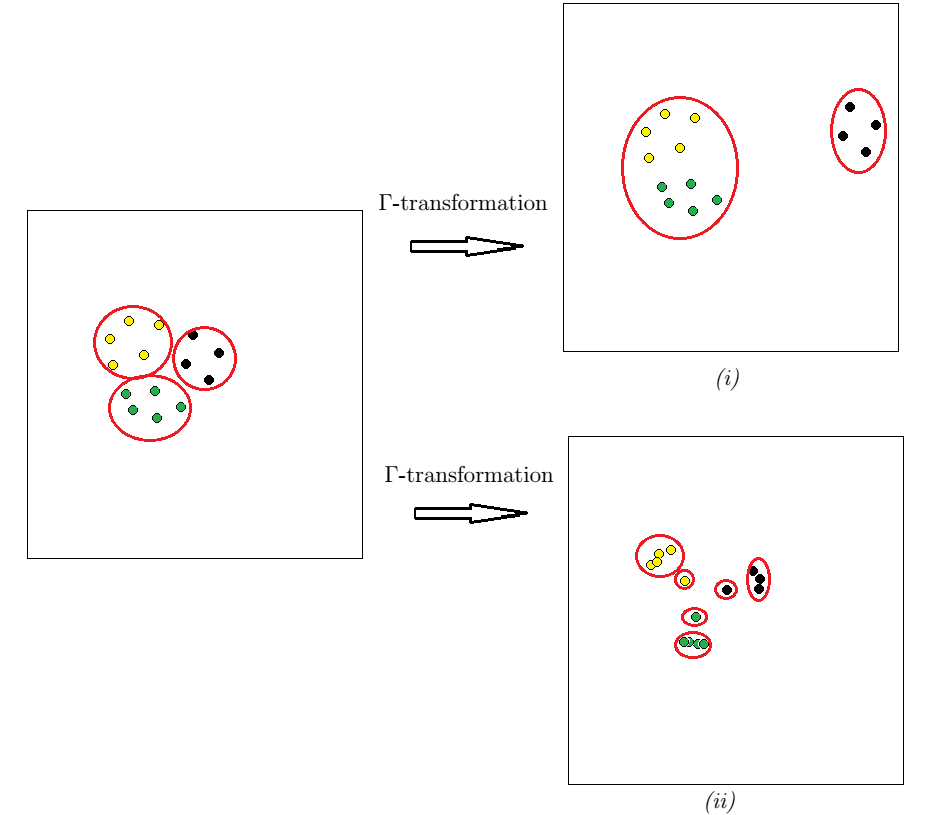
\includegraphics[width=0.65\textwidth]{Paper_figure_2.png}
 \end{center}
 \caption{\textit{This is the example of $\Gamma$-transformation which results in changing the structure of the data: In (i), one of the clusters is pulling away from the other two clusters significantly. In (ii), for each of the cluster, we the shrink all the points together but leave one point out.}}
 \label{fig:bsd2}
\end{figure}

Despite this seemingly reasonable assumption that $\Gamma$-transformation always keep the structure of the data the same, actually, in many cases (as \textit{Figure 2} shows), $\Gamma$-transformation will create undesirable transformation, in which the perturbed version of data should be clustered differently. For example, in (i), suppose we move one cluster infinitely away from other clusters, obviously it is a legitimate $\Gamma$-transformation, but the resulting data should be partitioned into  two clusters. However, consistency theorem, if hold, will require the clustering algorithm to produce three clusters as before. Similarly, in (ii), for each cluster, without breaking the constraints of $\Gamma$-transformation, if we shrink all the points together, but leave one points out, it should be more reasonable to partition the data in the way shown in \textit{Figure 2}.

These problems with consistency theorem motivate us to study the property of $\Gamma$-transformation, try to figure out in which case does $\Gamma$-transformation change the structure of the data set.
\section{A framework to investigate $\Gamma$-transformation} \label{sec:framework}
\subsection{Our approach} \label{subsec:approach}
We are taking a numerical approach to investigate how $\Gamma$-transformation change the structure of the data. The general idea is that suppose we have a dataset, we first apply some clustering algorithm on this dataset, which produce a partition $\Gamma$. Then, we apply $\Gamma$-transformation to this dataset for numerous times, and each time we will obtain a different dataset. For a clustering algorithm which doesn't satisfy consistency property, if we apply the algorithm to these $\Gamma$-transformed datasets, it should produce different partition results. We want to figure out what kind of $\Gamma$-transformation will result in partitions which are the same as the partition $\Gamma$ . To decide whether two partition results are the same, we need have some ``measurement", which could measure the difference between two partition, we will discuss various criteria to measure this difference in the third sub-section.

The implementation of these numerical analysis rely on the Python and several libraries including numpy, scikit-learn, etc. We enclose important part of code in Appendix \ref{app:calculations} (The full lists of code can be found on my personal  \href{https://github.com/Zehui127/clusteringResearch2019}{github page}).

\subsection{Generate data points by $\Gamma$-transformation} \label{subsec:blue}
Clustering algorithms can be classified into two groups by the types of required inputs: for algorithms like k-means, we will need the specific coordinates of the every points in the dataset, but for algorithm like single-linkage and k-medoids, they only need the distance functions as the input, then they can produce the partition results. To apply a $\Gamma$-transformation on the dataset with specific coordinates will be very difficult(actually it is computational impossible on any personal computer even small workspace, when the dataset become relatively big\footnote{Recall $\Gamma$-transformation require that we can only decrease the distance between the points within a cluster, and increase the distance between the point in different point. Suppose we have n points in the dataset, then when we move one point, we will need to exam $n-1$ equations to make sure our movement satisfy all the inequality. On the other hand, if we are working on the distance matrix, we don't need to worry about these constraints}). So we restrict our scope to the algorithms like single-linkage and k-medoids, which don't need the coordinates. Then in this case, to apply a $\Gamma$-transformation, we simply modify the distance function following the constraints of $\Gamma$-transformation.

With the scope restricted, a dataset containing $N$ data points can be denoted by a $N\times N$ distance matrix $X$, where $X_{i,j}$ refer to the distance between points $i$ and $j$, and it is symmetric matrix with diagonal elements equal to zero. Suppose we have a dataset $X$, a clustering function $f$, and $\Gamma = f(X)$. If we independently apply $\Gamma$-transformation to the dataset for $n$ time, we can obtain a set of distance matrices $D = \{X_1',X_2',\ldots , X_n'\}$, where each element $X_i'$ is the resulting distance matrix from a random $\Gamma$-transformation. Two things need to be noticed: First, every $X_i'$ is produced independently from $X$. Secondly, $\Gamma$-transformation from $X$ to $X_i'$ can make any changes to original distance matrix $X$, it is a completely random process. We enclose the python code of $\Gamma$-transformation in Appendix B, it is a function called \textbf{perturb\_distance\_matrix()}, which take the original distance matrix $X$ and partition $\Gamma$ as the input, and return a distance matrix produced from some random $\Gamma$-transformation.

What is the use of these distances matrices? Well, each of these distance matrices are produced from a ``$\Gamma$-transformation"; Among these transformations, some of the them will change the structure of the original dataset, in which case we expect to see that $f(X_i')\neq \Gamma$, while in the case where the structure of the dataset is preserved, we will expect $f(X_i')= \Gamma$.  Our aim is to target these good $\Gamma$-transformations among $D$, then try to come up with some quantities or models to capture these good $\Gamma$-transformations in the unseen cases. To identify ``good $\Gamma$-transformations", we will apply $f$ to all the elements of distance matrices $D$, which results in a set of new partition $P = \{\Gamma_1',\Gamma_2' \ldots \Gamma_n' \}$, where $\Gamma_i = f(X_i')$. We want to find all $i\in \{1,2\ldots n\}$ such that $\Gamma_i' = \Gamma$, but how can we compare two partitions? We will look at this problem in next section.

\subsection{Measure the difference between partition results} \label{subsubsec:red}
The task here is to compare two partitions of the same dataset, many criteria, such as Jaccard index, Variation of Information distance \cite{meilua2003comparing} and Rand index, can be used to describe the difference between two partitions. All these criteria follow a similar idea: the difference between two clusters is defined in terms of the number of points, or pairs of points two partition disagree \cite{von2010clustering}. In this paper, we will use an variation of a simple criteria - \textbf{Adjusted rand index} , this criteria is based on Rand index, but normalized to have better property. Let's first define Rand index.

Given a dataset of $n$ points $S = \{1,2\ldots n\}$ and two partition of $S$: $\Gamma=\{C_1,C_2\ldots \}$ and $\Gamma' = \{C_1',C_2'\ldots\}$, where $C_1,C_2\ldots$ and $C_1',C_2'\ldots\ $ are non-overlap subsets. 
	\begin{itemize}
\item Let $x =|S^*|$, where $S^*=\{(i,j)|i,j\in C_l$ and $i,j\in C_k' \}$
  
\item Let $y =|S^{**}|$, where $S^{**}=\{(i,j)|i\in C_{l_1},j\in C_{l_2}$ and $i\in C_{k_1}',j\in C_{k_2}' \} $
\end{itemize}
Rand Index, Rd, is defined as:
\begin{equation}
 Rd = \frac{x+y}{{n\choose 2}}
\end{equation}
${n\choose 2}$ is the total number of possible choices of pair. Rand index can be interpreted as the probability that $\Gamma$ and $\Gamma'$ will agree on a randomly chosen pair. The range of Rand index is $[0,1]$, when $Rd(\Gamma,\Gamma') =1$, $\Gamma$ and $\Gamma'$ are exactly the same, while $Rd(\Gamma,\Gamma') =0$ means two partition do not agree on any pair of points. However, Rand index is not often used directly, because it have two obvious drawbacks: For one, in practice, the value of Rand index is ususally in the range between $[0.5,1]$. Also, its baseline value can be high and does not take a constant value \cite{vinh2010information}. 

Due to these reasons, \textbf{Adjusted rand index} is introduced, it is proposed in 1985\cite{hubert1985comparing}. Adjusted rand index basically is a normalized version of Rand index, it is given by following formula:
\begin{equation}
 \textrm{Adjusted Rand Index} =  \frac{\textrm{Rand Index}-\textrm{Expected Rand Index}}{\textrm{Maximum Rand Index}-\textrm{Expected Rand Index}}
\end{equation}
Expected Rand Index is calculated by assuming the generalized hypergeometric distribution of randomness, we will not go into the details of this distribution. But after this normalization operation, Adjusted Rand index will be a better measurement for the difference between two clusters, it is bounded above by 1 and only equals to 1 if two partition are exactly the same, and close to zero when we randomly label the data into clusters. Furthermore, in practice, the value of the Adjusted Rand Index will be evenly ranging from 0 to 1.

In the simulation, we write our Rand Index function, but make use of the \textbf{Adjusted\_rand\_index()} function in sklearn library for efficiency purpose. Here is the graph showing the property of rand index and adjusted rand index.

\begin{figure}[H]
 \begin{center}
   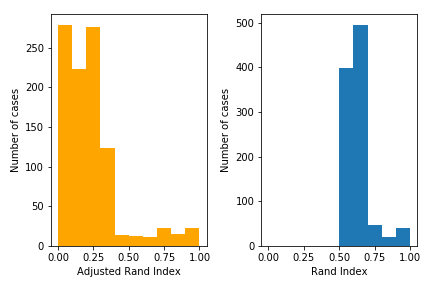
\includegraphics[width=0.4\textwidth]{adjusted.png}
 \end{center}
 \caption{\textit{We randomly generate 1000 pairs of partitions, then compute the Adjusted Rand Index and Rand Index for these pairs. It can be clearly seen that the value of Adjusted Rand Index is distributed across $[0,1]$, while Rand Index without Normalization concentrate on $[0.5,1]$}}
 \label{fig:bsd}
\end{figure}


\section{Simulation Results} \label{sec:red}
Following the framework proposed in section \ref{subsec:blue}, below is the simulation we did for investigating the property of $\Gamma$-transformation: We start from the original dataset, represented by distance matrix $X$, then let $\Gamma = f(X)$, where $f$ is the selected clustering algorithm we want to study. Apply $\Gamma$-transformation on $X$ for multiple times to get the perturbed version of dataset $D = \{X_1',X_2'\ldots X_n'\}$. Applying $f$ to every element of $D$ will result in a set of partitions $P = \{f(X_1'),f(X_2')\ldots f(X_n')\}=\{\Gamma_1',\Gamma_2' \ldots \Gamma_n' \}$. Finally, we calculate corresponding Adjusted Rand Index(ARI) for each of these partitions $\{ARI(\Gamma_1',\Gamma),ARI(\Gamma_2',\Gamma)\ldots ARI(\Gamma_n',\Gamma)\}$. \textit{Table-1} present the psudo-code for the simulation steps.

\begin{algorithm}
\label{algorithm}
    \caption{Simulation Process}
  \begin{algorithmic}[1]
    \INPUT Iteration time $n$, Clustering function $f$, Initial distance matrix $d_{origin}$
    \OUTPUT A Set containing $n$ Adjusted Rand Index $\{ARI_1,ARI_2\ldots ARI_n\}$, where $ARI_i = ARI(f(d_i),f(d_{origin}))$
	\STATE $i=1$    
    \STATE $\Gamma = f(d_{origin})$
    \WHILE{$i \leq n$}
      \STATE $d_i=\Gamma$-transformation$(d_{origin})$
      \STATE $\Gamma_i=f(d_i)$
      \STATE $ARI_i =$ AdjustedRandIndex$(\Gamma_i,\Gamma)$
      \STATE $i = i + 1$
    \ENDWHILE
  \end{algorithmic}
\end{algorithm}





\subsection{Simulation for K-mediods} \label{subsec: kmediods}


In the first experiment, $f$ is set to be \textbf{k-mediods}. We try $n=1000$, $n=10000$ and $20000$, \textit{Figure-4} shows the raw frequency of the Adjusted Rand Index in these cases, together with the Adjusted Rand Index under random perturbed data. Compared with the distribution of ARI upon random perturbed data which is the \textit{Figure-4}(a), the distribution of the ARI upon $\Gamma$-transformation clearly shows that $\Gamma$-transformation has the tendency to preserve the structure of the data. Even more remarkable, as $n \rightarrow \infty$, ARI tend to have a fixed \textbf{Probability Density Function}. In \textit{Figure-5}, We draw the density plot of the ARI when $n=10000,20000\ldots 70000$ (the density is estimated by the sum of multiple Gaussian distribution), and it shows that the density function tends to converge to the same function.
\begin{figure}[H]
 \begin{center}
   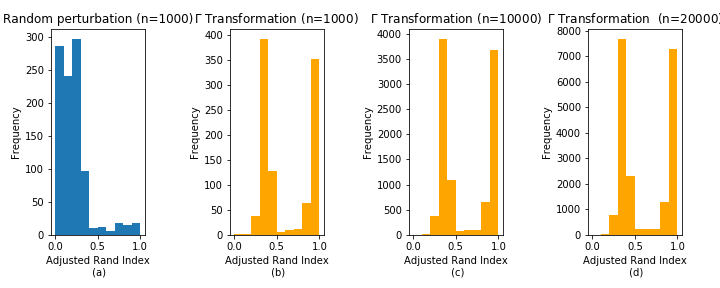
\includegraphics[width=0.7\textwidth]{simulate1.png}
 \end{center}
 \caption{\textit{Histogram of Adjusted Rand Index(ARI) for K-mediods. $n$ distance matrices $\{X_1',X_2'\ldots X_n'\}$ are created from $X_{origin}$ by $\Gamma$-transformation, $Y$ are created from random perturbation. (b),(c)and (d) shows histogram of $ARI(f(X_j'),f(X_{origin}))$ when $n=1000,10000,20000$ respectively.
(a) shows the histogram of $ARI(f(Y),f(X_{origin}))$ when $n =1000$.}}
 \label{fig:bsd}
\end{figure}

\begin{figure}[H]
 \begin{center}
   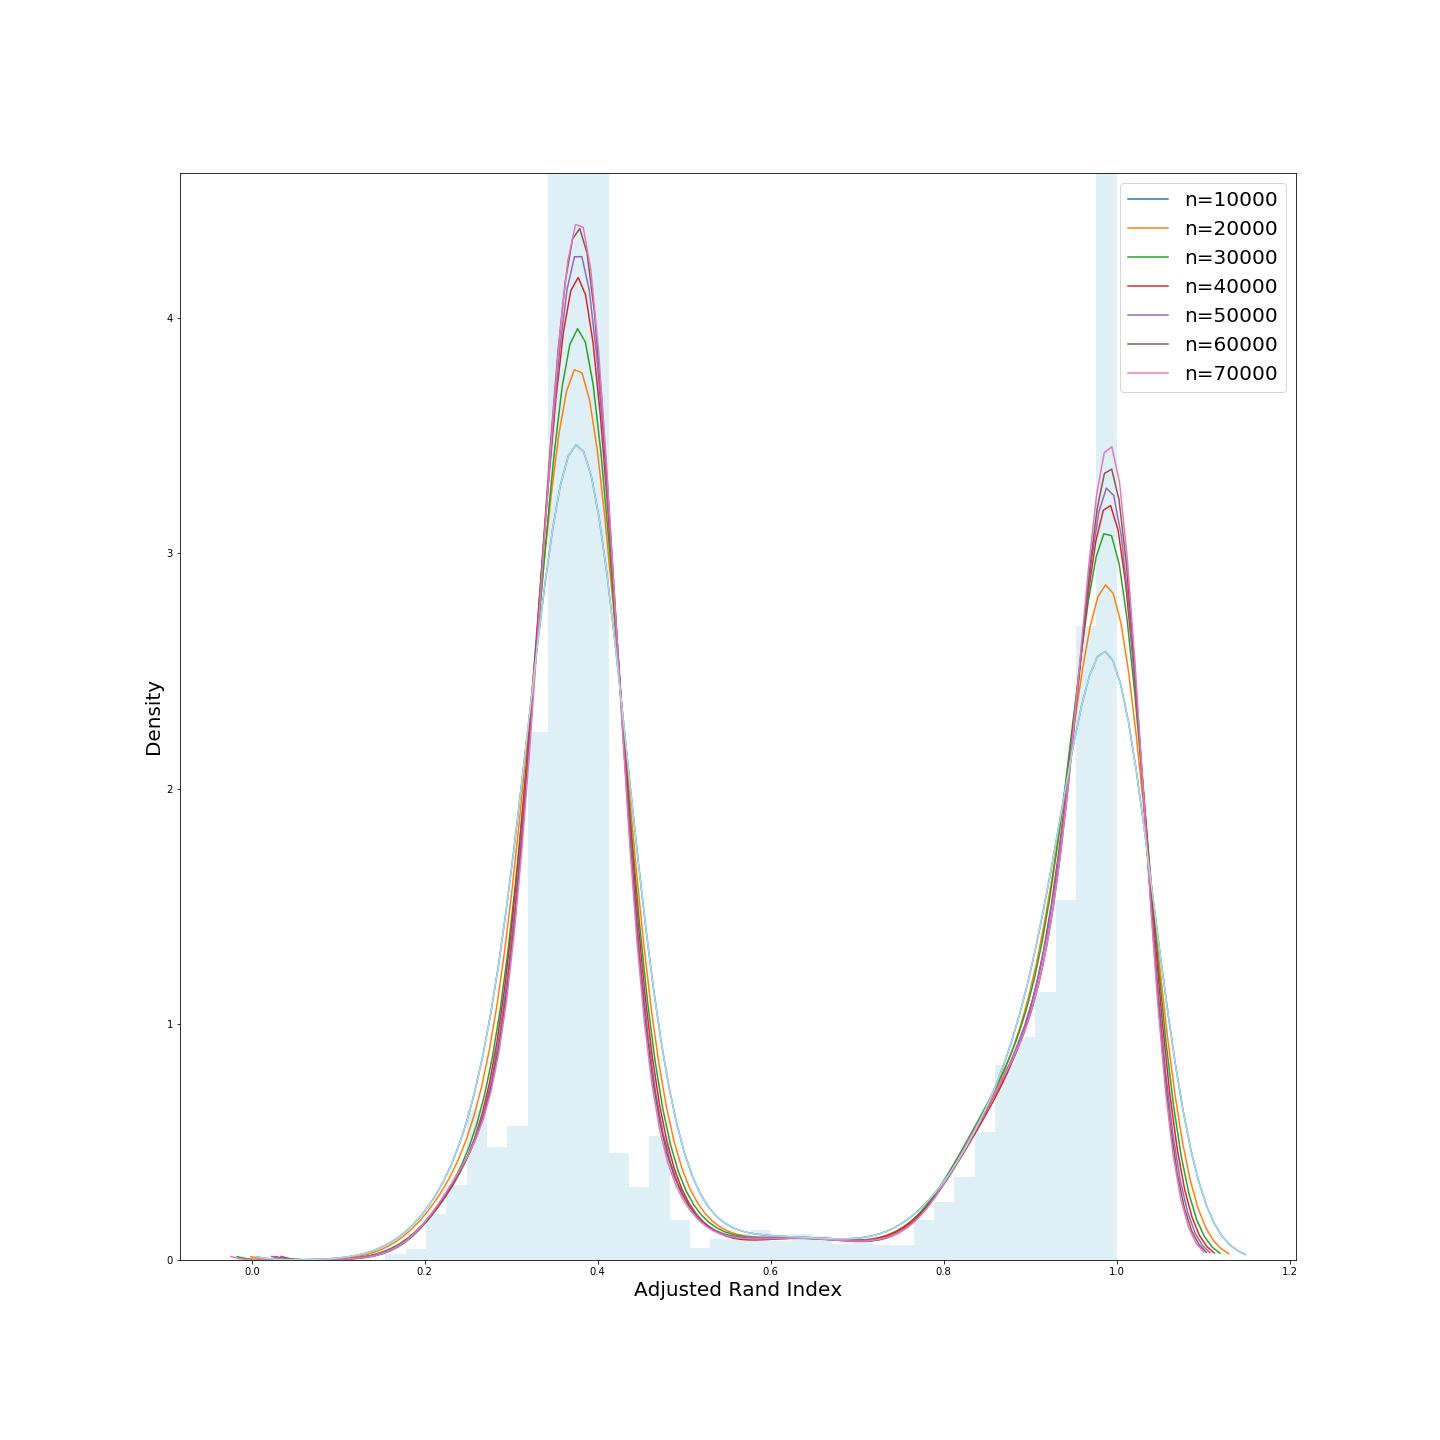
\includegraphics[width=0.7\textwidth]{simulate2.png}
 \end{center}
 \caption{\textit{We estimate the density function of $ARI(f(X_j'),f(X_{origin}))$ by the summing up Gaussian Distribution, this graph shows that as we increase the number of distance matrices, the density function converge to a ``true" density function.}}
 \label{fig:bsd}
\end{figure}

\subsection{Simulation for Complete Linkage} \label{subsec: Complete-linkage}
Complete-linkage is similar to Single-linkage Algorithm we discuss in the section \ref{subsec:Single-linkage}, it also take a bottom up approach - start from regarding each data points as a cluster, then merge two clusters with least dissimilarity\cite{christopher2008introduction}. But the dissimilarity is defined in following manner.
\begin{definition}
Let G,H represent two clusters, d is the distance function of the data set, then dissimilar $d_{SL}$ is defined as:
$d_{SL}(G,H) = \max_{i\in G,i'\in H}d_{ii'} $
\end{definition}
Here we let $f$ be Complete-linkage with k-clusters termination condition, and go through the same procedure as we did in previous section. \textit{Figure-\ref{fig:single-linkage}} shows the histogram of the ARI when $n=1000$ and $4000$. Compared to the histogram of K-mediods, it has heavier tail at $ARI = 1$, which could be interpreted as an evidence for that Complete-linkage are ``more consistency".  We also try to estimate the probability density function of ARI, but this time, instead of using mixture Gaussian Distribution, we assume the density function has a Gamma-distribution, then use the data to estimate the parameter of it. \ref{fig:single-linkage2} shows the estimated graph.

\begin{figure}[H]
 \begin{center}
   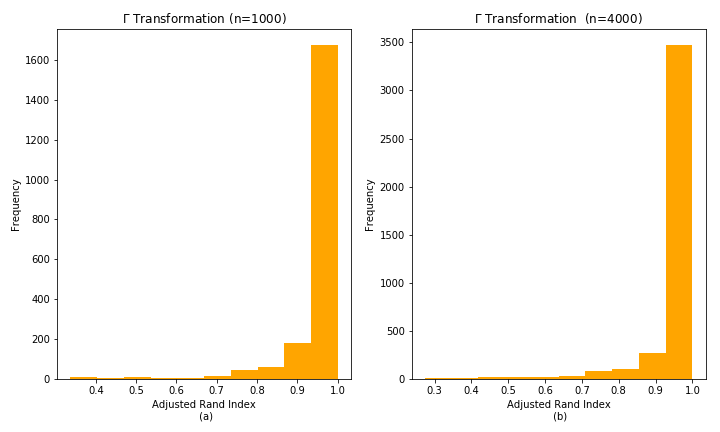
\includegraphics[width=0.7\textwidth]{simulate2_1.png}
 \end{center}
 \caption{\textit{Histogram of Adjusted Rand Index(ARI) for complete-linkage when $n=1000$ and $4000$ }}
 \label{fig:single-linkage}
\end{figure}

\begin{figure}[H]
 \begin{center}
   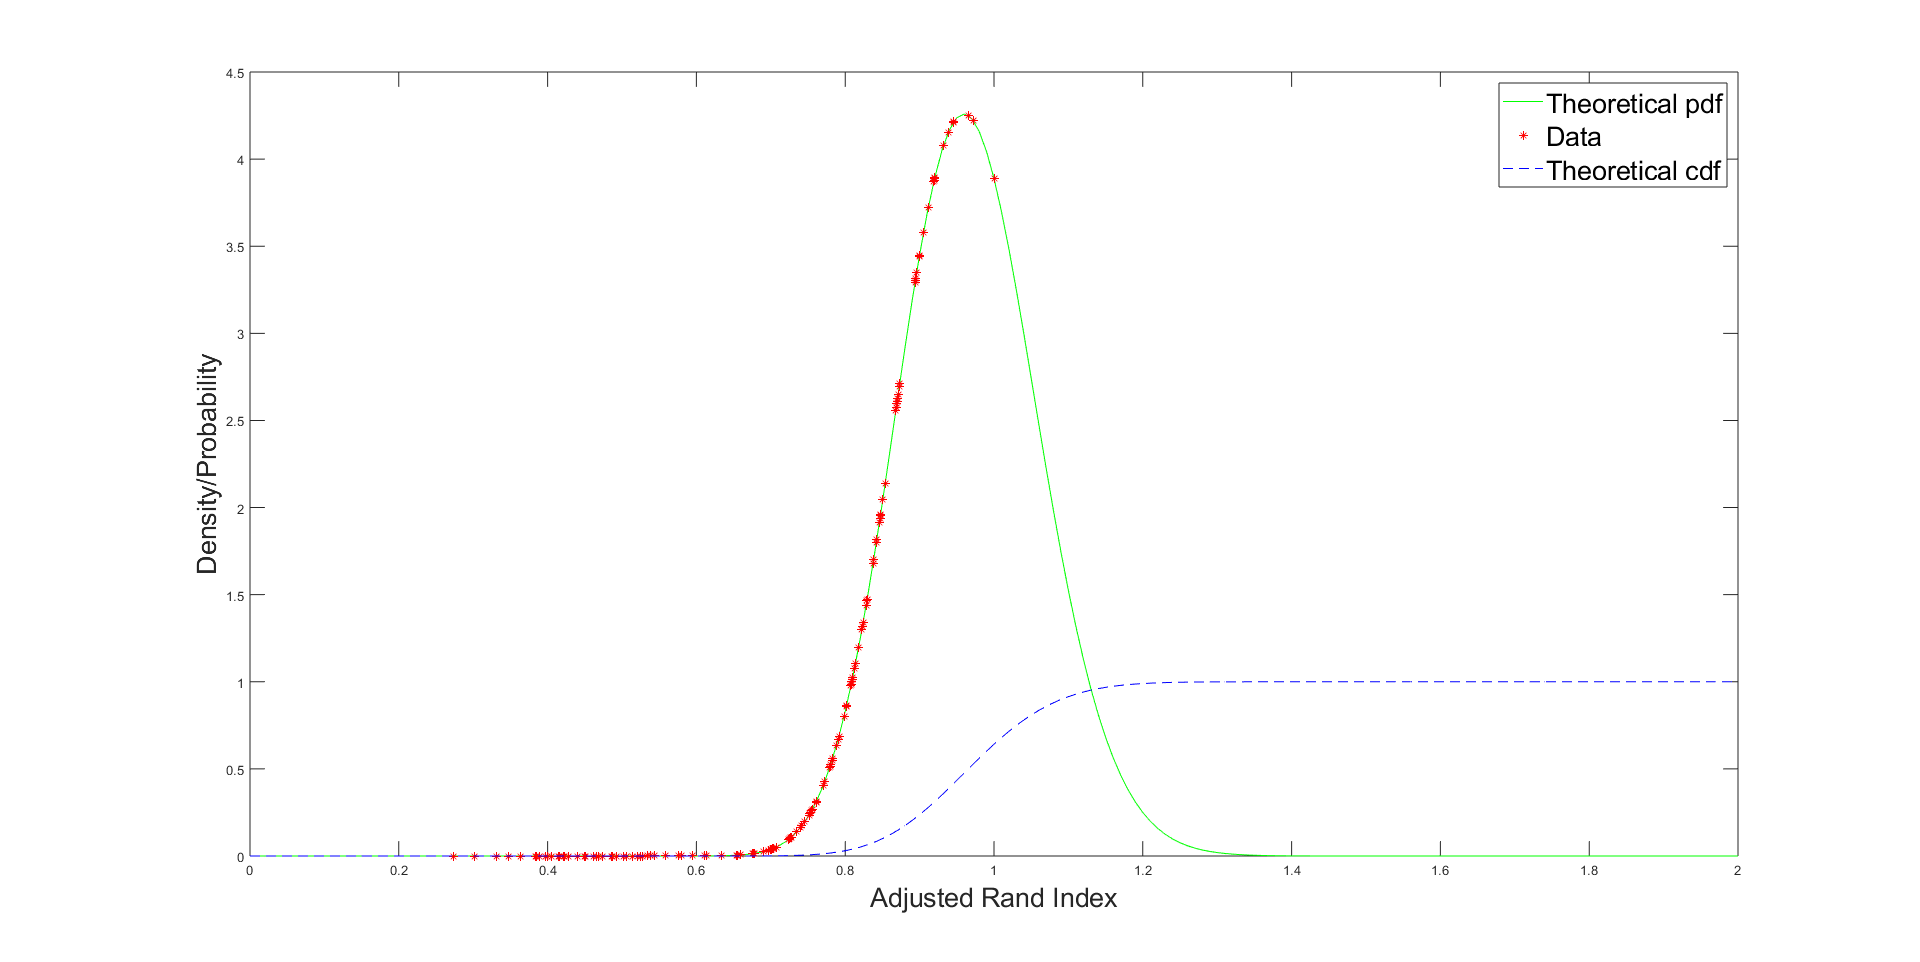
\includegraphics[width=1\textwidth]{Complete-linkage-cdf.png}
 \end{center}
 \caption{\textit{Estimated density function and cumulated density function of $ARI$ for Complete linkage}}
 \label{fig:single-linkage2}
\end{figure}

\subsection{Implication of the simulation} \label{subsec: simulationSum}
There are two important observations we get from the simulation process. The first one is that Adjusted Rand Index(ARI) after $\Gamma$-transformation had a very heavy tail at $ARI=1$, which is consistent with our intuition for $\Gamma$-transformation - it shouldn't change the structure of data set. The second observation is that different clustering algorithms will have different ARI distribution, for K-mediods, it has two 	``peaks" at ARI = 1 and ARI = 0.4, while for Complete-linkage, distribution of ARI can be fitted well by Gamma distribution. 

For Complete-linkage and K-mediods, $\Gamma$-transformation lead to a skewed distribution of ARI (The relative frequency of $ARI =1$ is higher than other value). Although we haven't tried all the clustering algorithm, it is reasonable to make the assumption that there are many other clustering algorithms satisfying this skewed distributed feature. So we formalize our assumption and state it as a refined version of consistency property, calling it \textbf{$\beta$-Partial Consistency}. 
Given $0<=\beta<=1$, it is defined as following:
\begin{definition}
$\beta $-Partial Consistency. Clustering algorithm $f$ satisfy $\beta$-Partial Consistency $\iff$ Given $D=\{d_1',d_2'\ldots d_n'\}$ contains $n$ uniformly sampled $\Gamma$-transformation of distance function $d$, as $n\rightarrow \infty$, there exists at least $\beta *n$ number of $d_i'\in D$ satisfying $f(d_i')=f(d)$ 
\end{definition}
Recall the original consistency property, it is actually a special case of $\beta $-Partial Consistency when $\beta = 1$. The original consistency property is a very strict one, only a small portion of clustering algorithm satisfy this property, but a wider range of clustering algorithms could satisfy $\beta$-Partial Consistency. From the simulation, we can see the potential existence of this property for \textbf{K-mediods} and \textbf{Complete-Linkage}. Figure-\ref{fig:single-linkage4} shows that the relative frequency of $ARI=1$ could tend to a fixed value as we increase the value of $n$.

\begin{figure}[H]
 \begin{center}
   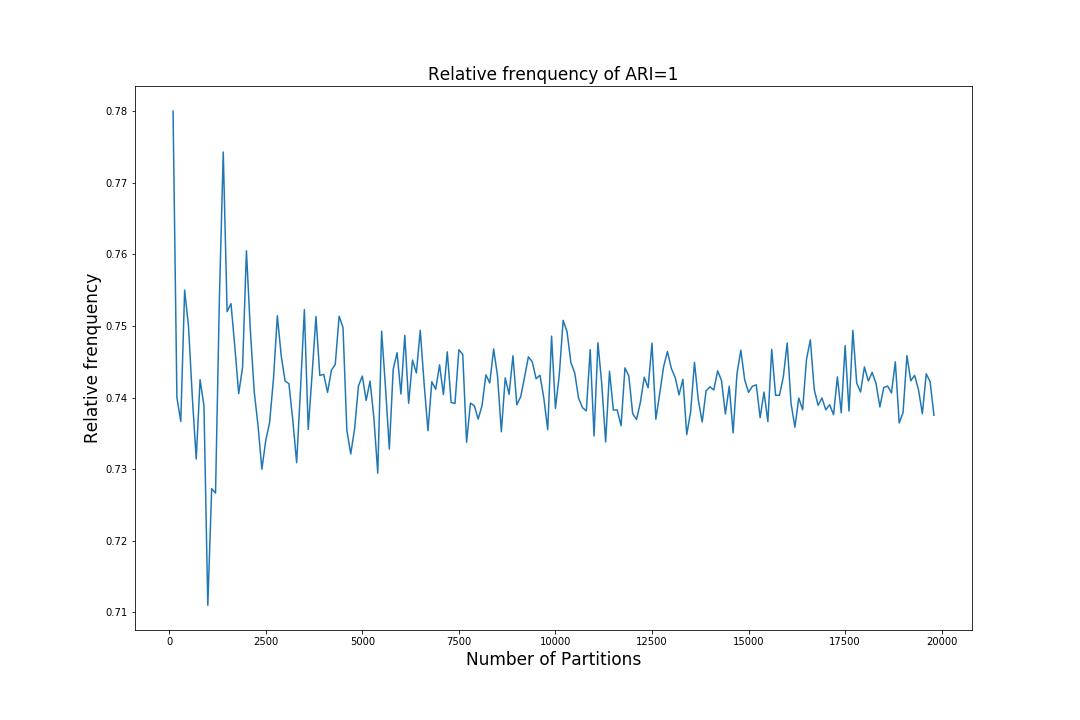
\includegraphics[width=0.7\textwidth]{convergence.png}
 \end{center}
 \caption{\textit{Change of the relative frequency of ARI = 1. Y-axis shows \textbf{relative frequency of} $1$ = $\frac{\textsl{Frequency of ARI}=1}{\textsl{Total number of cases}} $ for Complete-linkage algorithm; X-axis shows the value of n. As n increase, this value tend to a fixed value$=0.74$.}}
 \label{fig:single-linkage4}
\end{figure}


\section{Prediction With Machine Learning methods} \label{sec:Classification}


For the clustering algorithm without consistency, in many cases, they can still produce the same partition on the $\Gamma$-transformed dataset. We would like to know when these clustering algorithm could produce the same partition. Put it more formally, the problem is: Give $d'$ is the $\Gamma$-transformation of $d$, and particular clustering algorithm $f$, we would like to know whether $f(d)=f(d')$ holds without calculating $f(d)$ and $f(d')$. How can we do that? We solve this problem by regarding it as a canonical classification task in machine learning setting. Details of model building and model evaluation are given in the following subsections, we first give an example to show the application of the trained model.

Suppose we have a lot of datasets $\{d_1,d_2\ldots d_n\}$which need to be processed by a clustering algorithm, we know that all of these datasets are the $\Gamma$-transformation of Dataset $d$, the clustering algorithm don't satisfy consistency property, but satisfy Partial Consistency. By the assumption we made in section \ref{sec:red}, we know that many datasets will have the same  partition results as dataset $d$, if we have a classifier $C$, and it can tell us which dataset $d_i$ will have the same partition results as $d$, then we can skip these datasets. In this manner, we will save a lot of time and computation resources. Note, what motivate us to do this is the Partial Consistency assumption, if only a small amount of datasets have the same partition results as $d$, we will not bother using learning algorithm to train this model.

\subsection{Approach} 
\label{subsec:approach}
This method makes use of the simulation process from \textit{Section 4} to generate data. Given clustering algorithm $f$ and initial dataset $d$, where $d$ is the initial distance matrix of this dataset. we can use the simulation process to generate multiple $\Gamma$-transformation of $d$: $\{d_1,d_2\ldots d_n\}$, then calculate corresponding Adjusted Rand Index:$\{ARI(f(d_1),f(d)),$ $ARI(f(d_2),f(d))
\ldots  ARI(f(d_n),f(d))\}$. Now we have each pair $(d_i,ARI_i)$ as a training sample, to make it a classification problem, we convert the Adjusted Rand Index to Binary label using $\eta$ function, which is defined as following:
\[   
\eta(x) = 
     \begin{cases}
       0, &\quad x<1 \\
       1, &\quad x = 1 \\
     \end{cases}
\]
So formally, we have the training set $\{(d_1,\eta(ARI_1)),(d_2,\eta(ARI_2))\ldots (d_n,\eta(ARI_n))\}$. After fitting these data to various learning algorithms, we can obtain corresponding classifiers. 

We don't go into the details about learning algorithms, and the learning algorithm we used are decision tree, Support Vector Machine and Random Forest, which are all standard algorithms used in industry for small dataset.

\subsection{Implementation and Experiment Results} 
In the experiment, we use a dataset of 100 points, the distance between these points are represented by a $100\times100$ matrix. Using the Simulation Algorithm from section \ref{algorithm}, we obtain two datasets as the training set and test set, the size of training and test datasets are $40000$ and $10000$, respectively.
\subsubsection{Data Preprocessing} 
\label{subsec:Experiment}
For each sample $(d_i,\eta(ARI_i))$, $\eta(ARI_i)$ is either zero or one,  but $d_i$ is a $100\times100$ distance matrix, to fit it to the learning algorithm, we need to convert the distance matrix into a vector. Because the distance matrix is symmetric, we abandon the upper triangle of the distance matrix, so we get a vector of $5050$ dimensions. After the vectorization process, our distance matrix will looks like following: $\{(\vec{v_1},1),(\vec{v_2},0)\ldots (\vec{v_i},1)\}$, where $\vec{v_i}$ is a vector of $5050$ dimensions. 
\subsubsection{Results} 
After the preprocessing steps, we then fit the training set into the learning algorithm. For $f$=\textbf{K-medoid}, we fit the training set into Support vector machine, decision tree and Random forest, then test the performance of the trained model using the test set. Without any hyper-parameter tuning, SVM out perform the other two methods in terms of the \textit{average precision, recall} and \textit{f1-score}. We repeat the results for 4-times with different training set, figure \ref{fig:machine-learning} shows the performance of three algorithm in terms of average precision.

\begin{figure}[H]
 \begin{center}
   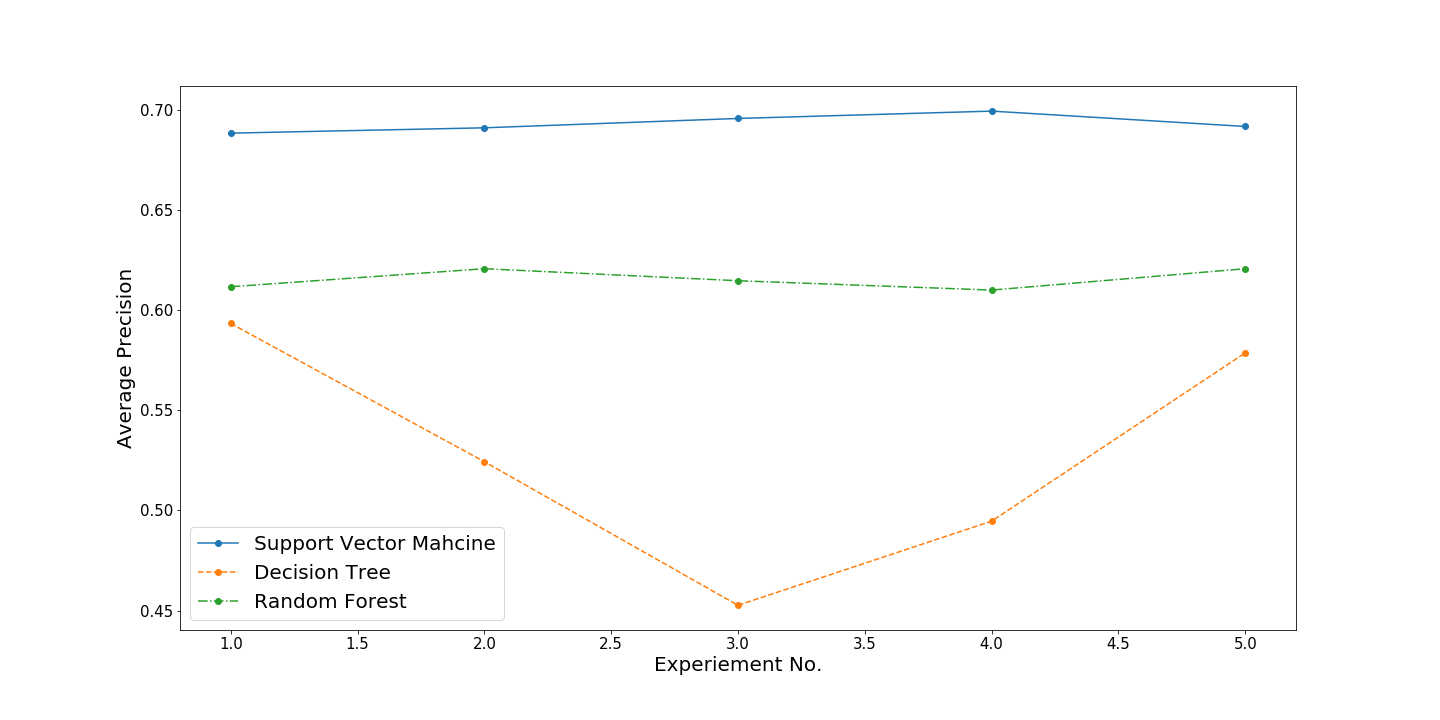
\includegraphics[width=0.7\textwidth]{posterDiscussion.png}
 \end{center}
 \caption{\textit{Average Accuracy of Support Vector Machine, Decision Tree and random Forest}}
 \label{fig:machine-learning}
\end{figure}

For $f=$\textbf{Complete Linkage}, we use Random Forest and Decision Tree to the training set, and it turns out Random Forest performed better this time, with average precision around $0.7$. The problem with these learning methods is that it usually performed very bad at the high dimension data, and require complex feature selection process, in our case, the data have 5050 dimensions! So a better way is to use deep learning model to deal with this high dimensional data, but due to the access to computation devices and time limits, we haven't try deep learning method. But we expect that with deep neural net, we could get much better performance. (All the code for training is available \href{https://github.com/Zehui127/clusteringResearch2019}{here.})




\section{Conclusions} \label{sec:conclusions}
In this paper, we have a complete review to the work of Kleinberg's work, and take a quantitative approach to study $\Gamma$-transformation and consistency. During the simulation, we make use of Adjusted Rand Index (ARI) to decide if two partition are the same, then identify the skewed distribution of ARI under $\Gamma$-transformation. Finally, We summarize  our observation as a property called Partial Consistency and make the assumption that there are many clustering algorithms satisfying Partial Consistency. 

We can think of partial consistency as a very weak version of consistency theorem, all the clustering algorithms satisfying original consistency will naturally satisfy partial consistency.  The future study could investigate what are the reasons behind this Partial Consistency. There are also other versions of consistency property, one recently published paper\cite{cohen2018clustering} focus on this problem as well. In that paper, they propose another consistency theorem called Refined Consistency, it basically states that if the $\Gamma$-transformation change the ``natural number of clusters" of original dataset, the clustering algorithm is still consistent even if it produce different  partition on the new dataset. In that case, for example, if Complete-linkage algorithm satisfy Refined Consistency, then we could reasonably deduce that $\Gamma$-transformation, in many cases, will not change the ``natural  number of clusters".


On the other hand, this simulation process has several limitations: First of all, we only work on two of the clustering algorithms, so the simulation results could differ for other clustering algorithm. Secondly, we haven't proved that these two algorithms satisfy \textbf{Partial Consistency}, currently, it is only an assumption from simulation results, and mean to provide a direction for future study. Thirdly, our python implementation of $\Gamma$-transformation can only deal with distance matrix but not specific coordinates due to the limitation of computational resources.
\newpage

\appendix

\section{Remaining Proofs for Single-linkage} \label{app:proof}
In this appendix, we provide the proof for \textit{Theorem \ref{second theorem}} and  \textit{Theorem \ref{third theorem}}.
\begin{proof}
\textit{theorem \ref{second theorem}}

\noindent Given data set $S$ and distance function $d$, and $f$ be the single-linkage with k-clusters termination condition. Scale-Invariance of $f$ is easy to prove, suppose another distance function $d'$ satisfies
\begin{equation}
\label{eq: myeq2.1}
	\forall i,j \in S, d'(i,j)=\beta d(i,j), \textsl{where} \beta >0
\end{equation}
Following the same idea of proof \ref{pf:myproof1}, Let 
\begin{equation}
\label{eq: myeq2.2}
\Gamma = f(S,d) = G_c(S,E)
\end{equation}
\begin{equation}
\Gamma' = f(S,d') = G_c'(S,E')
\end{equation}
If we can prove that edge sets $E=E'$, then $\Gamma = \Gamma'$ and scale invariance is proved.  
\begin{equation}
E = \{e_1,e_2\ldots e_m\}
\end{equation}
One key property of single linkage is that 
\begin{equation}
 d(e_i)<=d(e_k), \textsf{for } \forall e_i\in E, e_k\in E^\complement
\end{equation}
On the other hand, $E'$ is created by picking element with minimum  $d'(e)$ until k clusters are formed. By Equation \ref{eq: myeq2.1}, we have  
 \begin{equation}
 d'(e_i)<=d'(e_k), \textsf{for } \forall e_i\in E, e_k\in E^\complement
\end{equation}
So all the edges in $E$ have to be included in $E'$, and at this point, k clusters are formed, so the algorithm has to terminate. Thus, $E'$ contains the exactly the same elements as $E$, which means Scale-Invariance is proved.

The proof for consistency is more subtle. We first need to define what do we mean by equivalent Edge sets.
\begin{definition}
two edge sets $E_1$ and $E_2$ are equivalent $\iff$ $E_1$ and $E_2$ represent the same partition to the dataset. 
\end{definition}
Here is a example, in figure-\ref{fig:proof2}, $E_1=\{e_1,e_2,e_8,e_9\}$ and $E_2=\{e_2,e_5,e_7,e_8\}$ are \textbf{equivalent}, because both of them represent the same partition $\Gamma = \{\{1,2,3\},\{4,5,6\}\}$. 
\begin{figure}[H]
 \begin{center}
   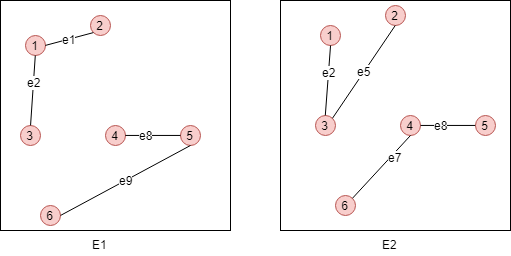
\includegraphics[width=0.6\textwidth]{proof.png}
 \end{center}
 \caption{\textit{$E_1$ and $E_2$ are two equivalent Edges sets}}
 \label{fig:proof2}
\end{figure}
Let $d''$ be the $\Gamma$-transformation of original distance function $d$, and $\Gamma_2 =f(S,d'') =G_c(S,E'')$. If we can prove that $E$ and $E''$ are a equivalent, then we will be able to prove $\Gamma'' = \Gamma$, thus the consistency of $f$.  With k-clusters termination condition, $f$ will continue to pick the edges with small weight until k sub-graphs $\{G_1^{sub},G_2^{sub}\ldots G_k^{sub}\}$are formed. Then all the edges can be classified into two groups: in the first group, the edges connect two nodes within the same sub-graph; in the second group, the edges connect two nodes belongs to different sub-graphs. Formally,
\begin{equation}
M = \{(i,j)|i,j\in G_l^{sub}\}
\end{equation}
\begin{equation}
M^\complement = \{(i,j)|i\in G_{l_1}^{sub},i\in G_{l_2}^{sub}\}
\end{equation}
Let $E=\{e_1,e_2\ldots e_m\}$, then we have $E\subseteqq M$ and 
\begin{equation}
\label{eq:cons1}
d(e_i)<=d(e_j), \quad \forall e_i\in E, e_j\notin E
\end{equation}
After the $\Gamma$-transformation, we will have 
\begin{equation}
\label{eq:cons2}
 d''(e_i)  >= d(e_i), \quad \forall e_i \notin M 
\end{equation}
Combine equation \ref{eq:cons1} and \ref{eq:cons2} we have 
\begin{equation}
\label{eq:cons3}
d''(e_i)>=d'(e_j),\quad \forall e_i \notin M, e_j\in E
\end{equation}
$E''$ will pick edges with small weight to include, but equation \ref{eq:cons3} indicate that edges which are not in $M$(the edges between clusters), can never be selected, because the by the time these edges are selected, the edges in $E$ either have been all included in $E''$, in that case, there are k clusters are formed, the selection process terminate,so $E=E''$, or the selection process terminate earlier, in this latter case, because no edges between the clusters are selected, $E''$ and $E$ have to be the equivalent Edges set to form k sub-graphs. Thus $\Gamma = \Gamma''$. The consistency is proved.
\end{proof}

\begin{proof}
\textit{theorem \ref{third theorem}}

We first prove richness, for a given Partition $\Gamma = G_c(S,E)$, where $E={e_1,e_2\ldots e_m}$. To make $f$ produce such a Edge set, we can simply define d as following:

\[   
d(e_i) = 
     \begin{cases}
       r, &\quad i\in\{1,2,3,\ldots m\} \\
       r+1, &\quad i\notin\{1,2,3,\ldots m\} \\
     \end{cases}
\]
Let $f(d) = G(S,E_{new})$. Because $f$ is the single-linkage with distance-r termination condition, it will put all the edges of weight smaller or equal to $r$ into Edge set, so $E_{new} = \{e_1,e_2\ldots d_m\} = E$

To prove the consistency of $f$, we can follow the same idea as we did in last proof. For Edges in $E$, we have 
\begin{equation}
d(e_i)>r, \quad \forall e_i\notin E
\end{equation}
And because of equation \ref{eq:cons3}, we have 

\begin{equation}
d''(e_i)>=d(d_i)>r \quad \forall e_i\notin M
\end{equation}
So these Edges connecting between the clusters can never be included in the Edge Set, On the other hand, we have 
\begin{equation}
d''(e_j)<=d(e_j)<=r \quad \forall e_i\notin E
\end{equation}
So $E$ have to at least include these edges, which form the same clusters as $\Gamma$, and whether or not include the other inter-connected edges will in $E''$ will not change the fact that $E''$ and $E$ are equivalent Edge set. So $\Gamma''=\Gamma$, we prove the consistency.
 
\end{proof}

\section{ Pyhton and Matlab code } \label{app:calculations}
Below is the code for $\Gamma$-transformation. We also enclose the matlab code for fitting the data to Gamma-distribution
\begin{lstlisting}[language=Python, caption=$\Gamma$-transformation()]
import numpy as np
import random
from math import factorial
# take the similarity matrix, partition result
def perturb_distance_matrix(in_matrix,partition):
    matrix = np.matrix.copy(in_matrix)
    #take the index of first,second ... cluster
    partition_list = list()
    for i in np.unique(partition):
        index_i = np.where(partition==i)
        if len(index_i[0])!=1:
            #In one cluster: Randomly select the x pair of points
            temp_upper_bound = factorial(len(index_i[0]))/(factorial(len(index_i[0])-2)*2)
            loop_time = random.randint(1,temp_upper_bound+1)
            #Randomly reduce the distance between each pair
            for j in range(1,loop_time+1):
                pair = np.random.choice(index_i[0],2,False)
                matrix[pair[0],pair[1]]=  matrix[pair[1],pair[0]]= random.uniform(0, 1)*matrix[pair[1],pair[0]]
            #store the partition into the list
        partition_list.append(index_i[0])
    #Ramdonmly select x' pair of clusters
    temp_upper_bound = factorial(len(partition_list))/(factorial(len(partition_list)-2)*2)
    loop_time = random.randint(1,temp_upper_bound+1)
    #increate the distance between clusters with a random ratio
    for i in range(1,loop_time+1):
        cluster_pair = random.sample(partition_list,2)
        #create a ramdom generated matrix - then do elementwise multiplication
        increase_coefficient = np.multiply((np.random.rand(cluster_pair[0].shape[0],cluster_pair[1].shape[0])+1),(np.random.randint(4,size=(cluster_pair[0].shape[0],cluster_pair[1].shape[0]))+1))
        temp_multiplier = np.multiply(matrix[np.ix_(cluster_pair[0],cluster_pair[1])],increase_coefficient)
        matrix[np.ix_(cluster_pair[0],cluster_pair[1])]= temp_multiplier
       # the points are symmetric to each other, so do the corresponding changes
        matrix[np.ix_(cluster_pair[1],cluster_pair[0])] = np.matrix.transpose(temp_multiplier)

    return matrix
\end{lstlisting}
\begin{lstlisting} [language=Matlab, caption=fitting the data to $\Gamma$ distribution]
% Fit gamma pdf to data
data = table2array(foo)
ab   = gamfit(data);
% Write the functional form of the pdf with the estimated parameters
a    = ab(1);
b    = ab(2);
gpdf = @(x) x.^(a-1)/(b^a*gamma(a)).*exp(-x/b);
% Plot the fitted pdf and the data
x    = 0:0.01:2;

plot(x,gpdf(x),'-g',data,gpdf(data),'*r',x,gamcdf(x,a,b),'--blue')
xx=xlabel('Adjusted Rand Index')
xx.FontSize = 20;
yy=ylabel('Density/Probability')
yy.FontSize = 20;
lgd=legend('Theoretical pdf','Data','Theoretical cdf')
lgd.FontSize = 20;
\end{lstlisting}


\newpage

\bibliographystyle{unsrt}
\bibliography{References}

\end{document}
